\documentclass[12pt]{article}

\usepackage{sbc-template}
\usepackage[brazil]{babel}
\usepackage{quoting}
\usepackage{setspace}
\usepackage{graphicx,url}
% \usepackage{cite}
%\usepackage{float}

\usepackage[utf8]{inputenc}  
\usepackage[alf]{abntex2cite}
%\usepackage[style=abnt,backend=biber]{biblatex}

\usepackage{enumitem}
\usepackage{caption}
\usepackage[section]{placeins} % impede que floats (tabelas/figuras) ultrapassem o limite da seção

\captionsetup{skip=2pt} % diminui o espaço entre legenda e tabela
\setlength{\textfloatsep}{8pt plus 2pt minus 2pt}
\setlength{\intextsep}{8pt plus 2pt minus 2pt}

\sloppy

\title{Título Principal}

\author{Dalton Solano dos Reis\inst{1}}

\address{Programa de Pós-Graduação em Computação Aplicada (PPGCAP)\\
Universidade do Estado de Santa Catarina (UDESC)
\email{dalton@furb.br}
}

\begin{document} 
% \makeatletter
% \renewcommand{\@cite}[2]{({#1\if@tempswa , #2\fi})}
% \makeatother


\maketitle

\begin{abstract}
Texto do Abstract.

\textbf{Keywords:} Palavra 1, Palavra 2, Palavra 3.
\end{abstract}
     
\begin{resumo} 
Texto do Resumo.

\textbf{Palavras chaves:} Palavra 1, Palavra 2, Palavra 3.
\end{resumo}

\section{Introdução} \label{sec:introducao}

Texto da Introdução. 

Mais Texto.

\section{Realidade Aumentada} \label{sec:aumentada}

Texto aqui.  

\section{Uso da Realidade Aumentada aplicada à Educação}\label{sec:aplicada}

Texto aqui (Figura \ref{fig:Fig_Cavalli2024}).

\begin{figure}[ht]
\centering
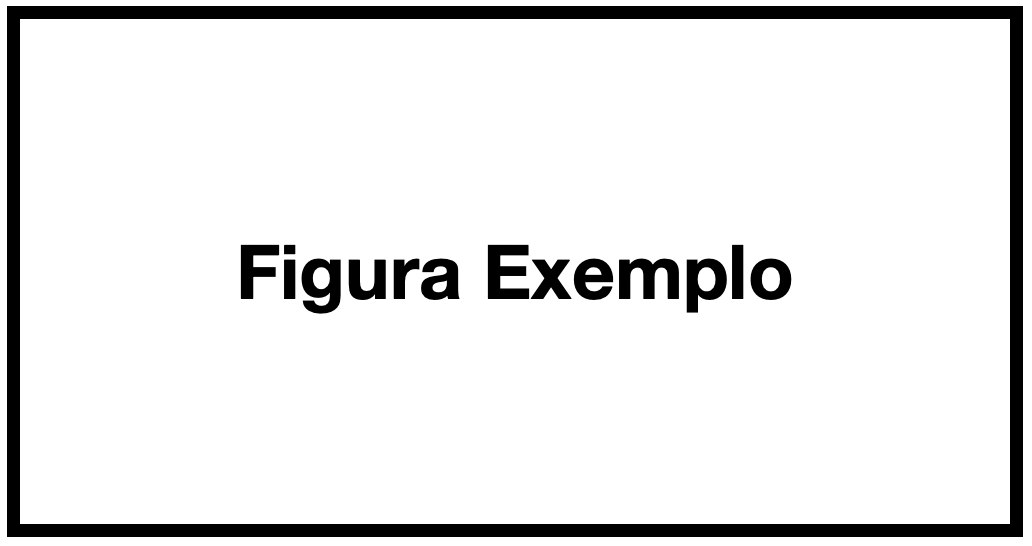
\includegraphics[width=.99\textwidth]{figura.png}
\caption{RA na Química: A) átomos $H_2O$ - B) elemento da água}
\label{fig:Fig_Cavalli2024}
\end{figure}

\section{Considerações Finais}\label{sec:finais}

Exemplo de citações.

Exemplo de \textbf{citação parentética} \cite{Teste2025}.

Segundo \citeonline{Teste2025}, esse é um exemplo de \textbf{citação narrativa}.

Somente o autor: \citeauthor{Teste2025}.

Somente o ano: \citeyear{Teste2025}.

% \bibliographystyle{sbc}

% --- Citações no padrão ABNT (NBR 10520) com abntex2cite ---
% Citação parentética: \cite{chave}  -> (AUTOR, ano)
% Citação narrativa:   \citeonline{chave} -> Autor (ano)
% Outros: \citeauthor{chave} (apenas autor), \citeyear{chave} (apenas ano)
\bibliographystyle{abntex2-alf}
\bibliography{bibliografia}
% \bibliography{../../../Dr/DR_Estudo}

\appendix
\renewcommand{\thesection}{Apêndice \Alph{section}}

% Apêndice A
\section{Um apêndice}\label{sec:apendA}

Somente o apêndice A.

% Apêndice B 
\section{Outro apêndice}\label{sec:apendB}

Mais um apêndice.

\end{document}
